\newcommand\tab[1][1cm]{\hspace*{#1}}

\section{Introdução}\label{sec}
\tab O presente trabalho tem como finalidade apresentar o resultado da Engenharia de Requisitos da Fábrica de Massas do Chef Nery. O empreendimento trata-se de uma micro empresa que fabrica diferentes tipos de massas.\\
\tab O contexto relacionado a necessidade do projeto é principalmente relacionado a necessidade de um melhor gerenciamento de clientes visando então buscar uma melhor forma de gerenciar seus pedidos e divulgar seus produtos.\\
\tab Para isso, é de fundamental importancia utilizar uma metodologia para o levantamento de requisitos e gerenciamento do processo em questão.\\
\tab Com uma análise acerca do contexto foi utilizado uma abordagem ágil composto de atividades do Scaled Agile Framework (SAFe). Com isso, foi possível desenhar o Processo de Engenharia de Requisitos contendo um também um modelo do Processo que será implementado no Trabalho 2.


\section{Contexto da Empresa (Chef Nery)} % (fold)
\label{sec:nova_sess_o}

\section{Justificativa da Abordagem}
\label{sec:nova_sess_o}

\section{Processo de Engenharia de Requisitos}
\label{sec:nova_sess_o}

\section{Elicitação de Requisitos}
\label{sec:nova_sess_o}

\section{Tópicos de Gerenciamento de Requisitos}
\label{sec:nova_sess_o}

\section{Planejamento do Projeto}
\label{sec:nova_sess_o}

\section{Ferramentas de Gestão de Requisitos}
\label{sec}
\tab Foi realizada uma pesquisa entre as ferramentas para gerir os requisitos, podendo elas serem versões Web ou de Desktop. Foram escolhidas então: Jira, Innoslate e Rally Dev.\\

\textbf{8.1 - Critérios}\\
\tab Para esta análise, foram listadas 5 características julgadas importantes para a gestão de requisitos para o projeto, referentes à Usabilidade, Rastreabilidade, Gestão de Mudanças, Flexibilidade e Licença.\\
\tab \textbf{Usabilidade:} Analisa se a usabilidade da ferramenta é de fato intuitiva ou não, o que pode vir a trazer contratempos para a equipe.\\
\tab \textbf{Licença:} Analisa a licença da ferramenta, caso seja grátis, paga, se possui isenção para projetos educativos, etc.\\
\tab \textbf{Rastreabilidade:} Analisa se é possível rastrear de forma eficaz a ferramenta.\\
\tab \textbf{Gestão de Mudanças:} Analisa quais são as funcionalidades que ajudam na gestão de mudanças, análise de impacto, e escopo.\\
\tab \textbf{Flexibilidade:} Analisa a flexibilidade de personalização da ferramenta ao contexto do projeto.\\

\section{Considerações Finais}
\label{sec:nova_sess_o}

\section{Referências}
\label{sec:nova_sess_o}




\onecolumn
\begin{usecase}
    \addtitle{Caso de Uso 1}{Exemplo de caso de uso}

    \addfield{Resumo:}{\lipsum[1]}

    \addfield{Ator Primario:}{Manolo}

    \addfield{Pré-condições:}{Aplicativo instalado}
\end{usecase}
\onecolumn

\onecolumn
\begin{figure}[h]
  \begin{center}
    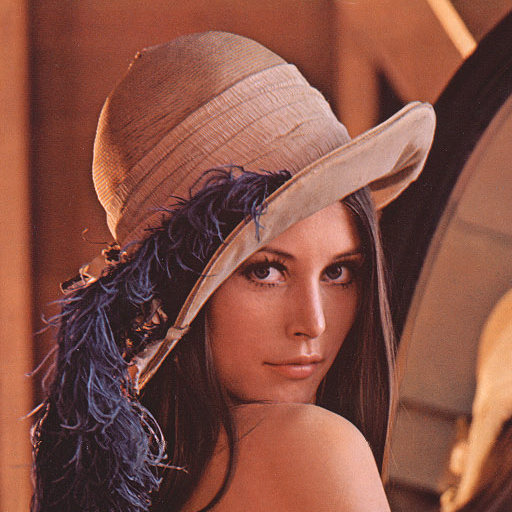
\includegraphics[width=0.8\textwidth]{conteudo/lena}
    \caption{Clássica Lena}
  \end{center}
\end{figure}
\onecolumn

\onecolumn

\begin{longtable}{  c  L{1.5cm}  C{1.2cm}  R{2.5cm}  p{2cm}  m{3.5cm}  }
\caption{Entidade: Motorista}\\
\toprule
Nome & Tipo & Tamanho  & Restrições de Domínio & Regra de Derivação & Observações \\ \midrule
\rowcolor[gray]{0.9}
CNH & Integer & 11 & - & - & Campo que armazena o número da CNH \\
Nome & Char & 30 & - & - & Campo que armazena o nome do motorista \\
\rowcolor[gray]{0.9}
CPF & Char & 20 & Somente números & - & Campo que armazena o número do CPF \\
RG & Char & 20 & Somente números & - & Campo que armazena o número de RG \\ \bottomrule
\end{longtable}

\onecolumn

